\begin{figure*}
    \centering
  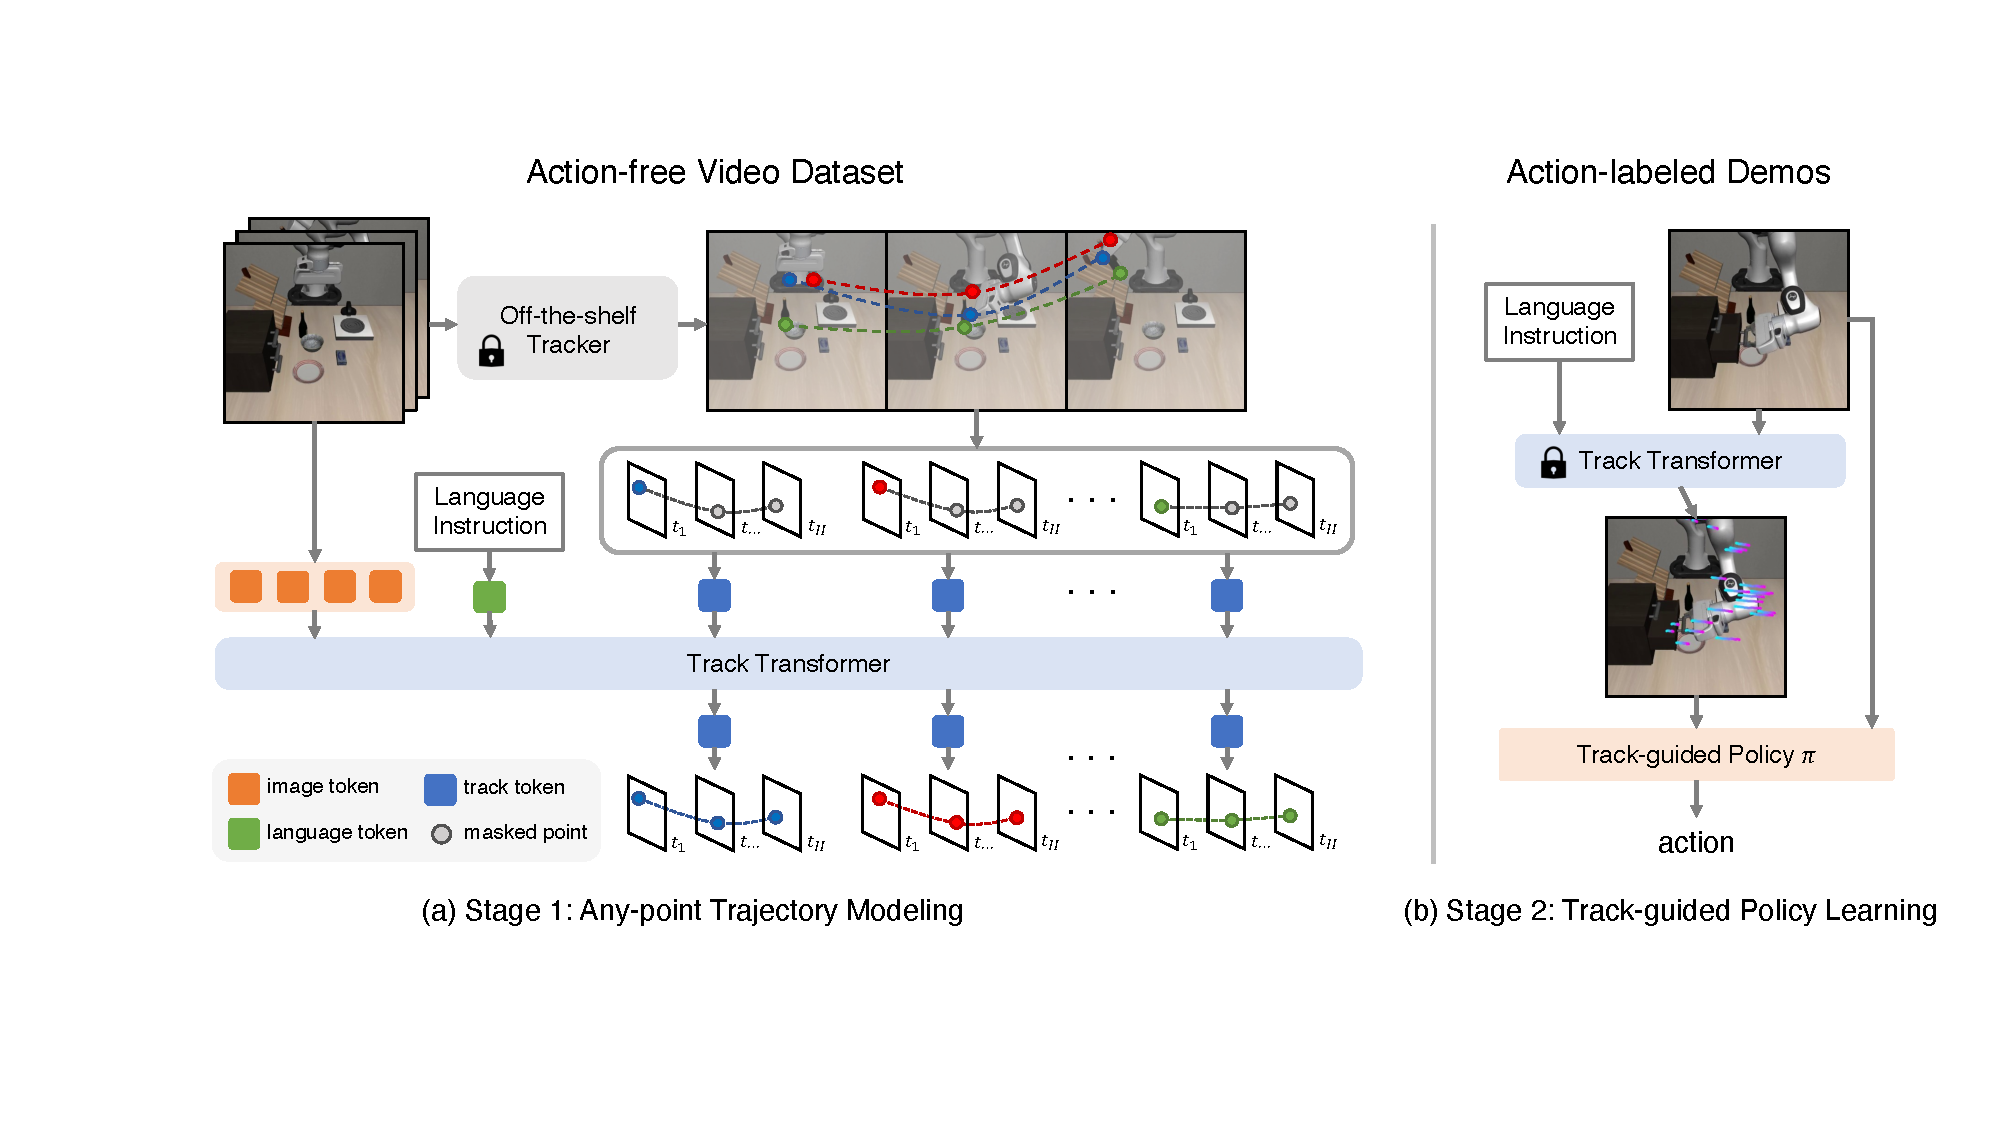
\includegraphics[width=\linewidth]{fig/system.pdf}
  \caption{Overview of our framework. (a) In the first stage, given an action-free video dataset, we first sample 2D points on one video frame and track their trajectories throughout the video using a pre-trained tracker. We then train a track transformer to predict future point trajectories given the current image observation, the language instruction, and the initial positions of the points. For the transformer input, we replace the future point positions with masked values. (2) In the second stage, we learn a track-guided policy to predict the control actions. Guidance from the predicted track enables us to learn robust policies from only a few action-labeled demonstrations. }
  \label{fig:system}
\end{figure*}


\section{Preliminary} \label{sec:prelim}
In this paper, we aim to learn robust control policies from a small set of action-labeled demonstration trajectories. Our central goal is to leverage the more scalable, unlabeled videos as a data source for pre-training. 

\noindent \textbf{Imitation from demos and videos.} To begin with, we denote the action-free video dataset as $\mathcal{T}_{o}=\{(\tau_o^{(i)}, \ell^{(i)})\}_{i=1}^{N_{o}},$ where $\ell^{(i)}$ is the language instruction for the $i^{th}$ episode and $\tau_o^{(i)} = \{o_t^{(i)}\}_{t=1}^T$ denotes the observation-only trajectory consisting of camera images. Similarly, we denote the demonstration dataset as $\mathcal{T}_{a}=\{(\tau_a^{(i)}, \ell^{(i)})\}_{i=1}^{N_{a}},$ where $\tau_a^{(i)} = \{o_t^{(i)}, a_t^{(i)}\}_{t=1}^T$ is the action-labeled trajectory. During imitation learning, our goal is to learn a policy $\pi_{\theta}$, parameterized by $\theta$ to mimic the expert behavior by the following behavioral cloning objective:
\begin{equation}
    \pi_{\theta}^{*} = \arg\min_{\theta} E_{(o_t,a_t, \ell)\sim \mathcal{T}_{a}}\Big[\mathcal{L}\Big(\pi_{\theta}(o_t, \ell), a_t\Big)\Big],
    \label{eq:bc}
\end{equation}
where $\mathcal{L}$ is the loss function, which could be Mean Squared Error (MSE) or cross-entropy loss.

\noindent \textbf{Tracking Any Point (TAP).} The recent advancements in video tracking~\cite{harley2022particle, doersch2023tapvid, doersch2023tapir, wang2023tracking, zheng2023pointodyssey} enable us to track the trajectory of each point in video frames without external supervision. In this paper, we utilize the off-the-shelf tracker proposed in~\cite{karaev2023cotracker}. Formally, given a sequence of images from a video $o_1, ..., o_T$, any one of the time steps $\bar{t} \in [1, T]$, and a set of points in that frame $\{p_{\bar{t}, k}\}_{k=1}^{K}$, where $p_{\bar{t}, k} = (x, y)$ is the point coordinate in the camera frame, the task of tracking is to predict the 2D camera-frame coordinates of the corresponding points in every frame $p_{t, k}$ where $t =1 \dots T$. In this paper, we use the terms \textit{trajectory} and \textit{track} interchangeably to refer to a sequence of 2D coordinates of any point, denoted as $(p_1, \dots, p_T)$. We only model the 2D trajectories in the camera frame so that we do not have to make additional assumptions about multi-view cameras, or the availability of depth, allowing future scaling to more diverse video datasets. The tracker additionally predicts a binary visibility value $v_{t, k}$ denoting whether the point is occluded at step $t$.

\section{Method}
Videos contain a great deal of prior information about the world, capturing physical dynamics, human behaviors, and semantics that are invaluable for policy learning. Beyond just learning representations from videos~\cite{sermanet2017tcn,nair2023r3m,ma2023vip}, we aim to learn a model from videos to predict future states for guiding a control policy. In this way, we can essentially decompose the visuomotor policy learning challenge into two parts. The first part is learning what to do next by generating future states as concrete \textit{sub-goals}, which is learned purely from videos. The second part is learning to predict control actions to follow the sub-goals, which require much less data to train compared to learning policies end-to-end. With sufficient video pre-training, we will be able to learn generalizable policies even from limited action-labeled trajectories. Prior works~\cite{du2023unipi,Ko2023Learning,black2023zero} have predominantly relied on pixel-level future frame prediction as video pre-training. While video prediction is resource-intensive during both training and inference stages, its focus on reconstructing pixel-level details, which are often extraneous to policy learning, can adversely affect the efficiency of subsequent policy learning.

We propose \textbf{A}ny-point \textbf{T}rajectory \textbf{M}odeling~(\textbf{ATM}). As illustrated in Figure~\ref{fig:system}, 
% ATM learns to predict future point trajectories in a video frame as the pre-training, then uses the predicted trajectories to guide policy learning. 
ATM is a two-stage framework: first learn to predict future point trajectories in a video frame as the pre-training with large-scale action-free videos, then use the predicted trajectories to guide policy learning with few-shot action-labeled demos. 
Our proposed method will be comprehensively detailed in this section: In Sec.~\ref{sec:track-model}, we first describe how to learn a point trajectory prediction model from an action-free video dataset $\mathcal{T}_{o}$. Then in Sec.~\ref{sec:track-policy}, we outline how we utilize the pre-trained track prediction model to learn a track-guided policy from a limited action-labeled trajectory datasets $\mathcal{T}_a$.

\subsection{Trajectory Modeling from Video Datasets} \label{sec:track-model}
Our goal is to pre-train a model from videos that forecasts the future point trajectories in a frame. More formally, given an image observation $o_t$ at timestep $t$, any set of 2D query points on the image frame $\mathbf{p}_t = \{p_{t, k}\}_{k=1}^K$, and a language instruction $\ell$, we learn a model $\mathbf{p}_{t:t+H} = \tau_\theta(o_t, \mathbf{p}_t, \ell)$ that predicts the coordinates of the query points in the future $H$ steps in the camera frame, where  $\mathbf{p}_{t:t+H} \in \mathbb{R}^{H \times K \times 2}$. To model the tracks, we propose a \textbf{track transformer} and illustrate the architecture in Figure~\ref{fig:system} (a).

\paragraph{Self-supervised Track Annotation.} \label{sec:TAP-annotation}
Initially, we generate point trajectories from action-free videos for trajectory modeling pre-training.
As described in Sec.~\ref{sec:prelim}, we employ a vision tracker to pre-process videos and generate a tracking dataset. For each video, we randomly sample a time step $\bar{t}$ and then randomly sample points on this frame and generate their tracks by running the tracker. However, for a static camera, most of the points that are sampled randomly will be in the background, thus providing little information when training our track transformer. To address this, we adopt a heuristic solution to filter out these static points: we first sample a grid of $n~\times~n$ on frame $\bar{t}$ and track the grid of points across the whole of the video to obtain an initial set of tracks $\tau \in \mathbb{R}^{n^2 \times T \times 2}$. Subsequently, we filter points that have not moved during the video by thresholding the variance of the point positions over time. In the final step, we resample points around the filtered locations and finally generate their positions using the tracker.

\paragraph{Multimodal Track Modeling.}
We formalize the future forecasting problem as a multi-modal masked prediction problem: we aim to predict the future positions of each point, conditioned on its current position, the current image observation, and a language instruction of the task. We first encode different modalities into a shared embedding space, each represented by a few tokens. For the tracks, we mask out the future positions of all points before encoding and then separately encode each point into one token. For the language instruction, we use a pre-trained BERT~\cite{devlin2019-bert} encoder. For the images, we split them into image patches and randomly masked out $50\%$ of the patches. We then pass all tokens through a large transformer model. Finally, we decode the track tokens into future trajectories of the corresponding points. Additionally, we reconstruct the image patches from the corresponding tokens following~\citet{he2022masked} as an auxiliary task, which we find useful for more complex tasks. Through this pre-training process, our track transformer learns the motion prior of particles within the video frames.


\subsection{Track-guided Policy Learning}\label{sec:track-policy}
After training a track transformer to predict future tracks based on observations, we can then learn policies guided by these predicted trajectories.

\paragraph{Arbitrary Points Tracking.} During track transformer pre-training, we can filter tracks without large movements. However, using this heuristic requires knowing the future positions of each point, which can be expensive to compute during policy inference. Instead, we find it sufficient to simply use a fixed set of 32 points on a grid for the policy. This sampling method avoids the potential complexities of learning key points or finding points to track~\cite{vecerik2023robotap} and works well in practice. ATM is permutation invariant to the input set of points, and we also find ATM to be robust to the distribution of the points, allowing us to use a different point sampling scheme from training for policy learning.

\begin{figure}[ht]
  \centering
  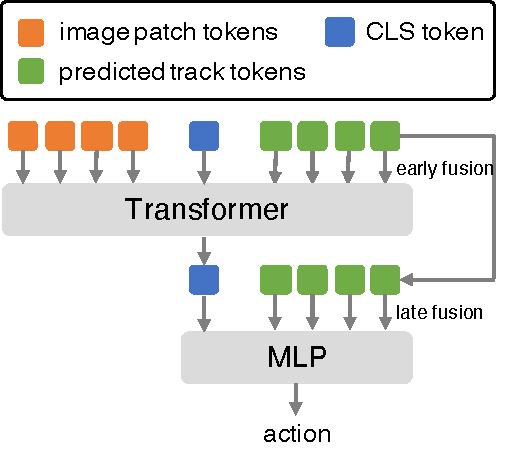
\includegraphics[width=.75\linewidth]{fig/simplified_track_policy.pdf}
  \caption{A visual illustration of the architecture of the track-guided policy. Given the current observation and the predicted tracks from the frozen pre-trained track transformer, we train a track-guided policy from a limited demonstration dataset.}
  \label{fig:track_policy}  
\end{figure}


\paragraph{Track-guided Policy Learning.} A track-guided policy $\pi(a_t | o_t, \textbf{p}_{t:t+H})$ takes input the current observation $o_t$ and the predicted tracks $\textbf{p}_{t:t+H}$ and predict the actions. A simplified illustration of our policy architecture is shown in Figure~\ref{fig:track_policy}. Our transformer policy architecture follows the architecture in prior works~\cite{liu2023libero, kim2021vilt}. Although the predicted tracks alone already provide rich information to predict the actions, we still incorporate contextual image observations into our policy so that no information is lost, as suggested in prior works~\cite{lin2023spawnnet}. We incorporate the track tokens both before and after fusion with the image tokens (early fusion and late fusion) to ensure that the guiding information from tracks can be effectively integrated. Surprisingly, as the tracks already provide the fine-grained subgoals, we find that the policy no longer needs language instruction at this stage as task specification. Essentially, the provided tracks have reduced the difficult policy learning problems into a much easier sub-goal following problems, reducing the policy into an inverse dynamics model. Our track-guided policy is trained with MSE loss. 
Note that, the weights of our policy model are randomly initialized rather than copied from the pretrained Track Transformer like other video-pretraining methods~\cite{nair2023r3m,ma2023vip}, because of the aim to separately study the task guidance capability of predicted trajectories.
A detailed architecture diagram and hyperparameters are available in the appendix.

